\documentclass{article}
\usepackage{graphicx} % Required for inserting images
\usepackage{amsmath}
\usepackage{multirow}
\usepackage{appendix}
\usepackage{float}
\usepackage{hyperref}
\usepackage[style=ieee]{biblatex}
\title{Anytime and Incremental Algorithms for Unknown Environments}
\author{Jeremy Kilbride\\ \texttt{jkilbrid@andrew.cmu.edu} 
\and Trevor Stack \\
\texttt{tstack@andrew.cmu.edu}
\and Evan Wassmann\\
\texttt{ewassman@andrew.cmu.edu}}
\addbibresource{project.bib}

\begin{document}

\maketitle

\begin{abstract}
    In this work, we seek to compare popular anytime and incremental algorithms for robot planning. Specifically, we explore the use of these algorithms for the case of a robot navigating in an unknown environment. The algorithms we explore include: A*, Anytime Repairing A*\cite{ara_star}, D* lite\cite{D_star_lite}, and Anytime D* \cite{anytimeD_star}. Our code can be found at \url{https://github.com/JeremyKilbride/Anytime_Dstar}.
\end{abstract}

\section{Motivation}
\quad With the rising demand for autonomous robotic systems, it is increasingly more valuable to understand the best algorithm for specific use cases. Often there are strict time constraints on planning; in environments known to be unchaining the robot path can be computed offline, but this is an unrealistic expectation. When unknown obstacles may be present, the environment is dynamic, or the execution of the robots moves are imperfect planning becomes a repeated task. In this work, we seek to explore which algorithms are most suitable for the task of a robot exploring an unknown environment. This is a common scenario when autonomous systems are used for exploration or surveillance tasks. In this case, the system needs to be able to recompute its path very quickly as it gathers more information about the world around it.  Common examples of this sort of task include: military surveillance, inspection in uncontrolled environments such as construction sites or warehouses, or autonomous driving in open spaces like parking lots. Many algorithms have been developed for this sort of fast recomputing, and in this work we selected three: Anytime Repairing A* (ARA*), D*lite, and Anytime D* (AD*). As a baseline we compared these to vanilla A*. We used several simulated scenarios to test and compare these algorithms. 

\section{Algorithms} \label{sec: Algos}
\quad We will now give a brief overview of each of the three algorithms we implemented for the task described above, along with details about our specific implementations of each algorithm.

\subsection{Anytime Repairing A*}
\quad The motivation behind Anytime Repairing A* is that returning an optimal path is often impossible due to the time constraints set on planning. This issue can be alleviated by performing multiple weighted A* searches with a decreasing weight value ($\varepsilon$). By doing this, the user can ensure that a path is returned, maintain sub-optimality bounds on the path, and, if time permits, improve the optimality of this path. Instead of replanning from scratch with each new $\varepsilon$, Anytime repairing A* uses the previously found g values (the cost to reach the state) and the previous open list to speed up the search. ARA* does this by keeping track of the previous open list, a list of "inconsistent states" or states whose cost value was lowered and have not been expanded since. When an inconsistent state is expanded, its inconsistency propagates to its children. States that were previously expanded and become inconsistent are not added to the open list when their g value is lowered, but are added to a separate list and used to initialize the open list for the next search along with the open list from the previous search. This is done because even if every state is restricted to being expanded once, the bounds on optimality hold. Each time $\varepsilon$ is decreased and a new search is to be initialized, the old open list must be reordered and the $f$ values of the states it contains must be recalculated, as the heuristic has changed. $\varepsilon$ is typically changed by small amounts each iteration to avoid expanding too many states. Our implementation of ARA* is based on the pseudocode shown in figure 3 of \cite{ara_star}.
\subsection{D* lite} \label{sec: D* lite}
\quad D* lite is an incremental graph search algorithm, which means that it is meant to quickly solve a series of similar searches by reusing information. More specifically, D* lite recomputes a plan when edge costs in the graph change. It does this by leveraging the idea of local consistency. Local consistency checks answer the following question: "does the current $g$ value of a state match what should be based on the $g$ values of its neighbors?". D* lite uses the $rhs$ value of a state to check local consistency. The $rhs$ value of a state is defined as follows:
$$
rhs(s)=\begin{cases}
   0 & \text{if} \: s=s_{goal}\\
   \min_{s^{'} \in Pred(s)}(g(s^{'})+c(s^{'},s)) & \text{otherwise}
\end{cases}
$$

During the actual search, the algorithm searches backward from the $s_{goal}$ to $s_{start}$ . For a robot moving on a grid, $s_{start}$ is set to the robot's current position. The algorithm is designed to only expand inconsistent states. A state is defined as inconsistent if $g(s) \neq rhs(s)$, further an inconsistent state is defined as over-consistent if $g(s) > rhs(s)$, and under consistent if $g(s) < rhs(s)$. In the case that the search finds an over-consistent state, it sets $g(s)=rhs(s)$, and updates the $rhs$ values of its neighbors. For an under-consistent state the search sets $g(s)=\infty$ and updates the $rhs$ values of that state and its neighbors. D* lite is able to efficiently recompute plans because it only expands inconsistent states that are relevant to the search. Our implementation of the algorithm is all in c++ and is modeled after the psuedocode shown in figure 3 of \cite{D_star_lite}. Our implementation makes heavy use of data structures in the c++ standard library in order to avoid issues with dynamic memory allocation as much as possible. For the open list, we do not use \texttt{std::priority\_queue}, but instead we use t\texttt{std::set}. This allows us to not only remove states from the top of the queue, but also to remove items from the middle of the queue, which allows us to strictly follow the original implementation of the algorithm. Our implementation could be optimized in a few ways. Firstly, we could implement our own version of a min heap that allows for removal from the top and the middle of the heap. This would allow for faster insertion and searching. Currently, we use a simple linear search when we search the open list for a given state. Apart from implementing our own data structure, we could also implement a more efficient search algorithm for searching the open list. Lastly, there are several optimizations shown in figure 4 of \cite{D_star_lite}, implementing these optimizations would also most make the algorithm more efficient.

\subsection{Anytime D*}

\section{Experiments}

\subsection{Experimental setup}
\quad We conducted experiments in multiple simulated environments in order to test the performance of our algorithm. In each environment, the robot starts out knowing its current state and the goal state and nothing about the environment. The environment is a 2D eight-connected grid map. Each cell in the map has a binary value showing if that cell is occupied or not. The cost for moving to any neighboring cell $s^{'}$ (diagonally or axis-aligned) is 1 if $s^{'}$ is unoccupied. If a neighboring cell $s^{'}$ is occupied, then the cost to move to that cell is $\infty$.  The robot also has a sensor range of $c$. This means that the robot "senses" the values of the cells within $\pm c$ of its current position in the $x$ and $y$ directions. Initially, the robot assumes all cells are unoccupied. After initializing the environment, the robot generates an initial plan. After the initial plan is generated, the robot follows the currently published plan until changes in the map are detected. When map changes are detected, the robot recomputes the plan and then continues moving toward the goal. The simulation terminates when the robot reaches the goal. An example of the maps used can be seen in figure \ref{fig:ex-map}. Other maps used for the simulated scenarios can be seen in appendix \ref{sec:maps}. For each environment, we run the simulation with the planners described in section \ref{sec: Algos} along with A* using a forward search as a baseline.

\begin{figure}[H]
    \centering
    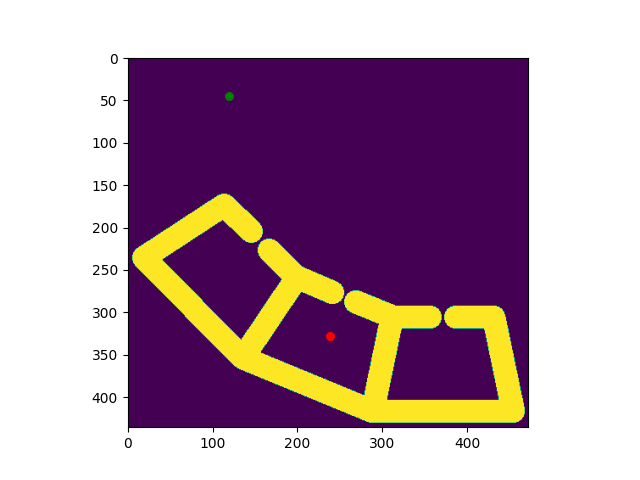
\includegraphics[width=0.8\linewidth]{new_map3.png}
    \caption{Visualzation of \texttt{new\_map3} used for robot navigation scenarios. Map size is $473 \times 436$. The green dot is the robot start, the red dot is the goal, yellow cells are occupied, purple cells are free.}
    \label{fig:ex-map}
\end{figure}

\subsection{Results and Discussion}
Figures \ref{fig:paths_A} and \ref{fig:paths_D} shows examples of the paths generated by our algorithms in the simulated environments. It is quite evident from these figures that the robot's overall path tends to be suboptimal since it does not have full knowledge of obstacles
\begin{figure}[h]
    \centering
    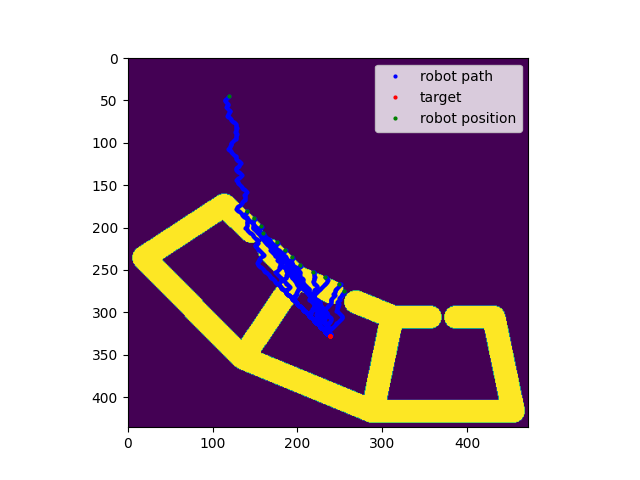
\includegraphics[width=0.6\linewidth]{map3_0_1.png}
    \caption{Paths generated as the robot moves in an unknown environment using the A* planner}
    \label{fig:paths_A}
\end{figure}
\begin{figure}[h]
    \centering
    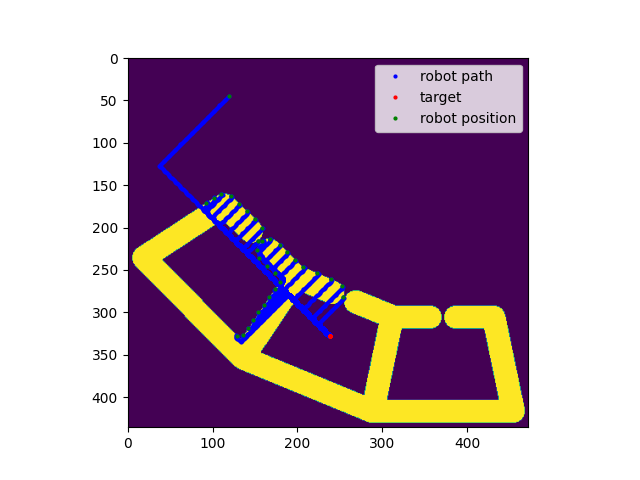
\includegraphics[width=0.6\linewidth]{map3_1_1.png}
    \caption{Paths generated as the robot moves in an unknown environment using the D* Lite planner}
    \label{fig:paths_D}
\end{figure}


\begin{table}[h]
    \centering
    \caption{Average number of states expanded per search}
    \begin{tabular}{|c|c|c|c|c|c|}
        \hline
        map                          &Sensor range & A*      &  ARA*       & D* Lite & AD* \\
        \hline 
\multirow{2}{*}{\texttt{new\_map1}}  &1            & 10,434.4&   3539.2    & 118.0   &  \\
                                     &5            & 12,836.5&   4104.9    & 104.4   &  \\
        \hline 
\multirow{2}{*}{\texttt{new\_map3}}  &1            & 1562.9  &  421.6      & 141.8   &  \\
                                     &5            & 1609.6  &  1401.7     & 136.5   &  \\
        \hline 
\multirow{2}{*}{\texttt{new\_map5}}  &1            & 1172.5  &  199.0     & 103.0   &  \\
                                     &5            & 1356.7  &  273.4     & 174.2   &  \\
        \hline 
\multirow{2}{*}{\texttt{new\_map8}}  &1            & 6864.2  &  235.6     & 290.8   &  \\
                                     &5            & 4027.0  &  554.6     & 223.8   &  \\
        \hline 
\multirow{2}{*}{\texttt{new\_map9}}  &1            & 3683.3  &  405.3     & 207.1   &  \\
                                     &5            & 4055.4  &  403.3     & 177.1   &  \\
        \hline
    \end{tabular}
    \label{table:states_expanded}
\end{table}


\begin{table}[h]
    \centering
    \caption{Number of steps taken by each planner, the optimal column shows the length of the path computed by A* with full knowledge of the map}
    \begin{tabular}{|c|c|c|c|c|c|c|}
        \hline
        map                          & sensor range&A*    &  ARA* & D* Lite & AD* & optimal\\
        \hline
\multirow{2}{*}{\texttt{new\_map1}}  & 1           &1313  &  1357     & 1100    &     & \multirow{2}{*}{421} \\
                                     & 5           &1337  &  1307     & 1347    &     &  \\
        \hline 
\multirow{2}{*}{\texttt{new\_map3}}  & 1           &316   &  1067    & 608     &     & \multirow{2}{*}{283}\\
                                     & 5           &554   &  633     & 600     &     & \\
        \hline 
\multirow{2}{*}{\texttt{new\_map5}}  & 1           &214   &  224     & 249     &     & \multirow{2}{*}{199}\\
                                     & 5           &230   &  223     & 199     &     & \\
        \hline 
\multirow{2}{*}{\texttt{new\_map8}}  & 1           &596   &   419    & 410     &     & \multirow{2}{*}{410}\\
                                     & 5           &591   &   415    & 410     &     & \\
        \hline 
\multirow{2}{*}{\texttt{new\_map9}}  & 1           &376   &   599    & 551     &     & \multirow{2}{*}{350}\\
                                     & 5           &375   &   396    & 551     &     & \\
        \hline
    \end{tabular}
    \label{table:steps}
\end{table}

\begin{table}[h]
    \centering
    \caption{Average time (ms) taken to compute a single plan by each planner}
    \begin{tabular}{|c|c|c|c|c|c|}
        \hline
        map                         &sensor range & A*    &  ARA*    & D* Lite & AD* \\
        \hline
\multirow{2}{*}{\texttt{new\_map1}} & 1           & 7.25 &    8.75   & 5.10     &     \\
                                    & 5           & 7.61 &    10.54  & 5.84     &     \\
        \hline           
\multirow{2}{*}{\texttt{new\_map3}} & 1           & 0.80 &    0.82   & 3.02     &     \\
                                    & 5           & 0.58 &    2.94   & 3.42     &     \\
        \hline
\multirow{2}{*}{\texttt{new\_map5}} & 1           & 0.54 &  0.40     & 2.19     &     \\
                                    & 5           & 0.64 &  0.528    & 3.09     &     \\
        \hline
\multirow{2}{*}{\texttt{new\_map8}} & 1           & 3.26 &    0.60   & 7.62     &     \\
                                    & 5           & 1.26 &    1.20   & 5.93     &     \\
        \hline
\multirow{2}{*}{\texttt{new\_map9}} & 1           & 1.79 &   0.897    & 7.41     &     \\
                                    & 5           & 1.26 &   0.864    & 6.98     &     \\
        \hline
    \end{tabular}
    \label{table:time}
\end{table}

Tables \ref{table:states_expanded}-\ref{table:time} show the results of running our planners in 5 different environments. For these experiments we set the sensor range to 1 and 5. Additionally, for all simulations we set the max planning time for ARA* to 10ms. By this we mean that each time we call ARA* the algorithm will decrease $\varepsilon$ as much as possible within 10 ms. One result that is consistent across all algorithms is that as the sensor range is increased, the number of states expanded in a single planning episode increases. This is because the robot is receiving more information about the environment at each step, so at any given time in the simulation with a range of 5 the map that the robot has will have as many or more obstacles as would be the case with a range of 1. Thus, for any given time in the simulation, the robot within the greater sensor range will expand as many or more states as the robot with the lower range, since the robot with the greater range has discovered more obstacles.  It can be seen from Table \ref{table:states_expanded} that D* lite expands significantly fewer states each time it re-plans compared to A* or ARA*; however, in our case re-planning from scratch with A* or ARA* is often faster because the data structures we used for the open list are different between the algorithms. In our A* and ARA* implementations the open list is a \texttt{std::priority\_queue}, whereas the open list in D* lite is a \texttt{std::set}. As discussed in section \ref{sec: D* lite}, using a \texttt{std::set} for the open list is quite inefficient and could be improved with a more custom implementation of a min heap. We believe that more efficient data structures would allow D* lite to beat A* not only in number of states expanded but also in computation time. Further we see that sometimes the robot makes more moves when using the D* lite planner when compared to A*. This stems from the fact that the two algorithms reconstruct the path in slightly different ways. A* uses back pointers to the best predecessor, whereas D* lite uses a backward search and calculates the best successor as $\text{argmin}_{s^{'} \in Succ(s)} (c(s,s^{'})+g(s^{'}))$. In the case where two or more neighbors of a state have equal $g$, the two algorithms will most likely break the tie in different ways. This seems to cause the algorithms to take different paths around obstacles, which can clearly lead to highly suboptimal behavior when the robot only has partial knowledge of the environment.   

\section{Conclusion}
\quad In this work, we compared three different algorithms that can be used for efficiently re-planning in unknown environments. All of these algorithms exhibit some amount of suboptimal behavior when the environment is only partially known, which can be seen in table \ref{table:steps}. Overall, we find that the best algorithm is really dependent on the application. We find that for very cluttered environments, the D* lite is the best since it is able to reuse a vast majority of previously computed states. This is evident when looking at the statistics from Tables \ref{table:states_expanded} and \ref{table:time} for the \texttt{new\_map1} environment. This environment has lots of obstacles, and D* lite expands $\sim$ 100 times fewer state, resulting in faster computation, even with the inefficiencies of our specific D* lite implementation. On the other hand, for cases where keeping planning time within a certain limit is critical, we find that the anytime algorithms (ARA* and AD*) are more well suited to the task.



\printbibliography

\appendix
\section{Maps} \label{sec:maps}
\begin{figure}[H]
    \centering
    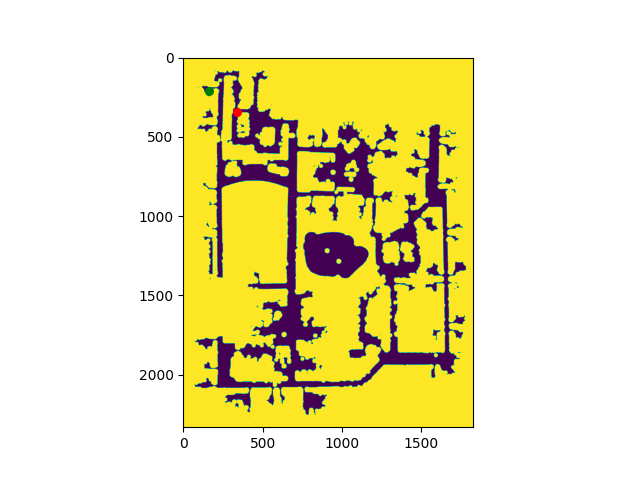
\includegraphics[width=0.8\linewidth]{new_map1.png}
    \caption{visualization of \texttt{new\_map1}, map size is $1825 \times 2332$ }
    \label{fig:map1}
\end{figure}

\begin{figure}[H]
    \centering
    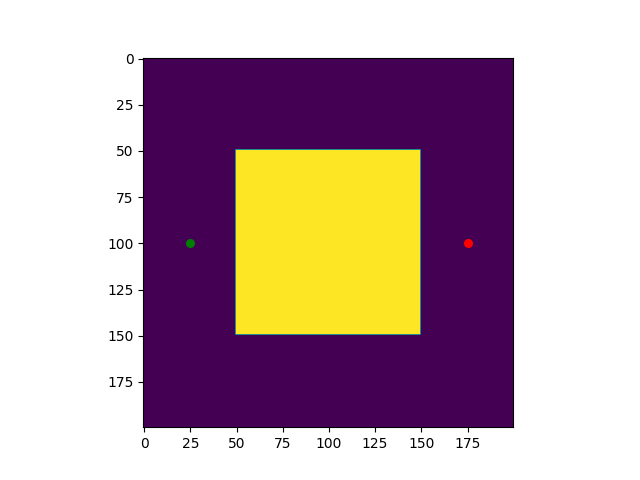
\includegraphics[width=0.8\linewidth]{new_map5.png}
    \caption{visualization of \texttt{new\_map5}, map size is $200 \times 200$ }
    \label{fig:map5}
\end{figure}
\begin{figure}[H]
    \centering
    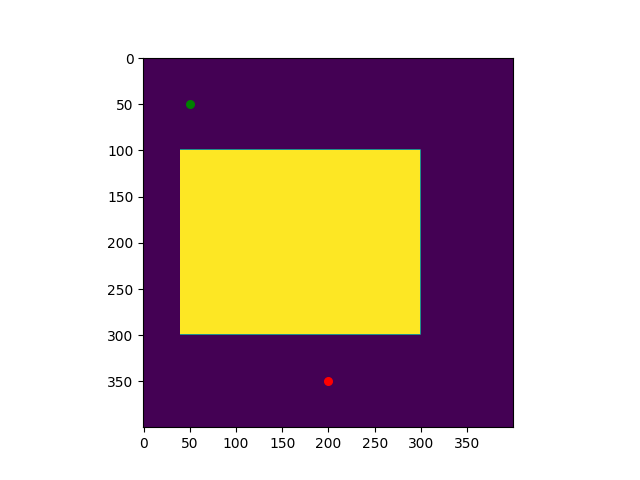
\includegraphics[width=0.8\linewidth]{new_map8.png}
    \caption{visualization of \texttt{new\_map8}, map size is $400 \times 400$ }
    \label{fig:map8}
\end{figure}
\begin{figure}[H]
    \centering
    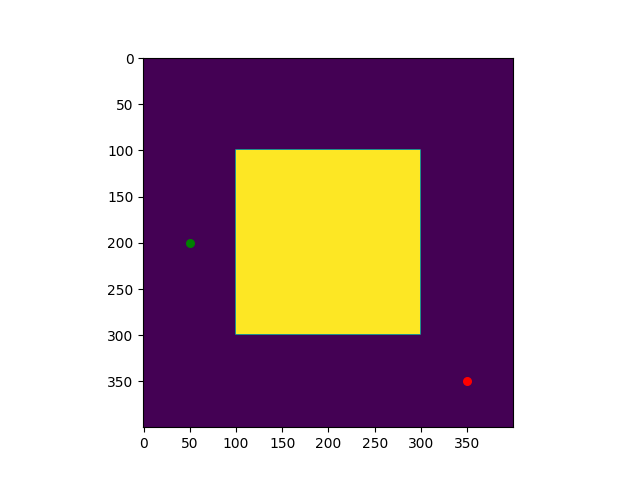
\includegraphics[width=0.8\linewidth]{new_map9.png}
    \caption{visualization of \texttt{new\_map9}, map size is $400 \times 400$ }
    \label{fig:map9}
\end{figure}

\end{document}
